% Schmidt decomposition at bond n: the bond index caps the rank (Session 4).
% Own drawing (Fable). Compile with: pdflatex schmidt_cut.tex ; result moves to ../schmidt_cut.pdf
\documentclass[11pt,tikz,border=3pt]{standalone}
\usepackage{amsmath,amssymb}
\usepackage{xcolor}
\definecolor{coursedark}{HTML}{1B2A4A}
\definecolor{courseaccent}{HTML}{7A2E8C}

\begin{document}
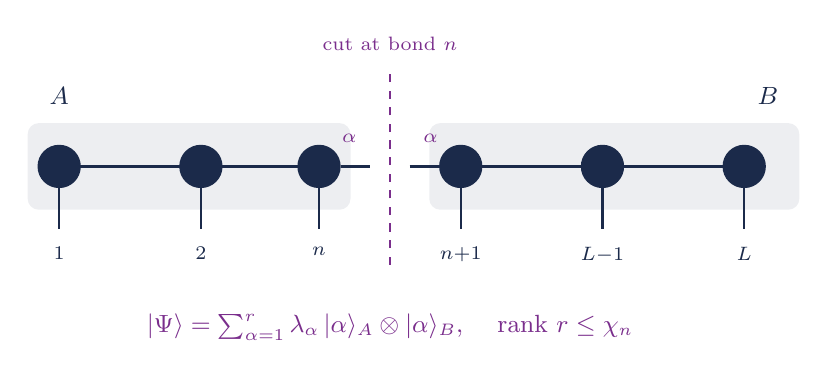
\begin{tikzpicture}[
    mps/.style={circle, fill=coursedark, inner sep=0pt, minimum size=5.5mm},
    wire/.style={draw=coursedark, line width=0.8pt},
    lbl/.style={font=\small, text=coursedark, align=center},
    idx/.style={font=\scriptsize, text=coursedark, align=center},
  ]

  % blocks A and B
  \fill[coursedark!8, rounded corners=4pt] (-0.40,-0.55) rectangle (3.70,0.55);
  \fill[coursedark!8, rounded corners=4pt] (4.70,-0.55) rectangle (9.40,0.55);
  \node[lbl] at (0.0,0.90) {$A$};
  \node[lbl] at (9.0,0.90) {$B$};

  % sites, physical legs down (same orientation as the MPS chain figure)
  \foreach \x/\s in {0/1, 1.8/2, 3.3/n, 5.1/{n{+}1}, 6.9/{L{-}1}, 8.7/L} {
    \node[mps] at (\x,0) {};
    \draw[wire] (\x,-0.275) -- (\x,-0.80);
    \node[idx, anchor=north] at (\x,-0.90) {$\s$};
  }
  \draw[wire] (0,0) -- (3.3,0);
  \draw[wire] (5.1,0) -- (8.7,0);

  % severed bond with exposed index alpha on both stubs
  \draw[wire] (3.575,0) -- (3.95,0);
  \draw[wire] (4.45,0) -- (4.825,0);
  \node[idx, text=courseaccent, anchor=south east] at (3.90,0.18) {$\alpha$};
  \node[idx, text=courseaccent, anchor=south west] at (4.50,0.18) {$\alpha$};

  % the cut
  \draw[courseaccent, dashed, line width=0.9pt] (4.2,-1.25) -- (4.2,1.25);
  \node[idx, text=courseaccent, anchor=south] at (4.2,1.35) {cut at bond $n$};

  % Schmidt form annotation
  \node[lbl, text=courseaccent, anchor=north] at (4.2,-1.75)
    {$|\Psi\rangle=\sum_{\alpha=1}^{r}\lambda_\alpha\,|\alpha\rangle_A\otimes|\alpha\rangle_B$,
     \quad rank $r\le\chi_n$};
\end{tikzpicture}
\end{document}
